% questions.tex —— 2004 年·全国卷Ⅱ·理科 · 题目内容片段（无答案）
% 由 tools/generate_projects.py 依来源总账自 2004/2004_数学真题_全国2理_试题.md 生成，勿手改（改源 MD 后重跑）


\gkpart{数学}

\begin{gktip}
\textbf{来源说明}：本题面依据固定源 PDF 两页 A3 题面逐题转录，原卷印刷页码 186–187。固定源不附答案，答案和解析均由本库独立复算。

\textbf{图形说明}：第 20 题的原卷图形关系重绘为 TikZ/PGFPlots 矢量图。图形标记所指的 PNG 不随仓库保存。
\end{gktip}

\gkpart{一、选择题}

\begin{question}
\gkti{1}已知集合 $M=\{x\mid x^2<4\}$，$N=\{x\mid x^2-2x-3<0\}$，则集合 $M\cap N=$\mbox{（　　）}

（A）$\{x\mid x<-2\}$　　（B）$\{x\mid x>3\}$　　（C）$\{x\mid-1<x<2\}$　　（D）$\{x\mid2<x<3\}$

\end{question}
\begin{question}
\gkti{2}$\displaystyle\lim_{x\to1}\dfrac{x^2+x-2}{x^2+4x-5}=$\mbox{（　　）}

（A）$\dfrac12$　　（B）$1$　　（C）$\dfrac25$　　（D）$\dfrac14$

\end{question}
\begin{question}
\gkti{3}设复数 $\omega=-\dfrac12+\dfrac{\sqrt3}{2}i$，则 $1+\omega=$\mbox{（　　）}

（A）$-\omega$　　（B）$\omega^2$　　（C）$-\dfrac1\omega$　　（D）$\dfrac1{\omega^2}$

\end{question}
\begin{question}
\gkti{4}已知圆 $C$ 与圆 $(x-1)^2+y^2=1$ 关于直线 $y=-x$ 对称，则圆 $C$ 的方程为\mbox{（　　）}

（A）$(x+1)^2+y^2=1$　　（B）$x^2+y^2=1$　　（C）$x^2+(y+1)^2=1$　　（D）$x^2+(y-1)^2=1$

\end{question}
\begin{question}
\gkti{5}已知函数 $y=\tan(2x+\varphi)$ 的图象过点 $\left(\dfrac\pi{12},0\right)$，则 $\varphi$ 可以是\mbox{（　　）}

（A）$-\dfrac\pi6$　　（B）$\dfrac\pi6$　　（C）$-\dfrac\pi{12}$　　（D）$\dfrac\pi{12}$

\end{question}
\begin{question}
\gkti{6}函数 $y=-e^x$ 的图象\mbox{（　　）}

（A）与 $y=e^x$ 的图象关于 $y$ 轴对称

（B）与 $y=e^x$ 的图象关于坐标原点对称

（C）与 $y=e^{-x}$ 的图象关于 $y$ 轴对称

（D）与 $y=e^{-x}$ 的图象关于坐标原点对称

\end{question}
\begin{question}
\gkti{7}已知球 $O$ 的半径为 $1$，$A\text{、}B\text{、}C$ 三点都在球面上，且每两点间的球面距离为 $\dfrac\pi2$，则球心 $O$ 到平面 $ABC$ 的距离为\mbox{（　　）}

（A）$\dfrac13$　　（B）$\dfrac{\sqrt3}{3}$　　（C）$\dfrac23$　　（D）$\dfrac{\sqrt6}{3}$

\end{question}
\begin{question}
\gkti{8}在坐标平面内，与点 $A(1,2)$ 距离为 $1$，且与点 $B(3,1)$ 距离为 $2$ 的直线共有\mbox{（　　）}

（A）$1$ 条　　（B）$2$ 条　　（C）$3$ 条　　（D）$4$ 条

\end{question}
\begin{question}
\gkti{9}已知平面上直线 $L$ 的方向向量 $\boldsymbol e=\left(-\dfrac45,\dfrac35\right)$，点 $O(0,0)$ 和 $A(1,-2)$ 在 $L$ 上的射影分别是 $O_1$ 和 $A_1$，则 $\overrightarrow{O_1A_1}=\lambda\boldsymbol e$，其中 $\lambda=$\mbox{（　　）}

（A）$\dfrac{11}{5}$　　（B）$-\dfrac{11}{5}$　　（C）$2$　　（D）$-2$

\end{question}
\begin{question}
\gkti{10}函数 $y=x\cos x-\sin x$ 在下面哪个区间内是增函数\mbox{（　　）}

（A）$\left(\dfrac\pi2,\dfrac{3\pi}2\right)$　　（B）$(\pi,2\pi)$　　（C）$\left(\dfrac{3\pi}2,\dfrac{5\pi}2\right)$　　（D）$(2\pi,3\pi)$

\end{question}
\begin{question}
\gkti{11}函数 $y=\sin^4x+\cos^2x$ 的最小正周期为\mbox{（　　）}

（A）$\dfrac\pi4$　　（B）$\dfrac\pi2$　　（C）$\pi$　　（D）$2\pi$

\end{question}
\begin{question}
\gkti{12}在由数字 $1,2,3,4,5$ 组成的所有没有重复数字的 5 位数中，大于 $23145$ 且小于 $43521$ 的数共有\mbox{（　　）}

（A）56 个　　（B）57 个　　（C）58 个　　（D）60 个

\end{question}
\gkpart{二、填空题}

\begin{question}
\gkti{13}从装有 3 个红球、2 个白球的袋中随机取出 2 个球，设其中有 $\xi$ 个红球，则随机变量 $\xi$ 的概率分布为：

\nopagebreak[4]
\[
\begin{array}{c|ccc}
\xi&0&1&2\\
\hline
P&&&
\end{array}
\]

\end{question}
\begin{question}
\gkti{14}设 $x\text{、}y$ 满足约束条件

\nopagebreak[4]
\[
\begin{cases}
x\geqslant0,\\
x\geqslant y,\\
2x-y\leqslant1,
\end{cases}
\]

则 $z=3x+2y$ 的最大值是\gkblank{}。

\end{question}
\begin{question}
\gkti{15}设中心在原点的椭圆与双曲线 $2x^2-2y^2=1$ 有公共的焦点，且它们的离心率互为倒数，则该椭圆的方程是\gkblank{}。

\end{question}
\begin{question}
\gkti{16}下面是关于四棱柱的四个命题：

① 若有两个侧面垂直于底面，则该四棱柱为直四棱柱；

② 若两个过相对侧棱的截面都垂直于底面，则该四棱柱为直四棱柱；

③ 若四个侧面两两全等，则该四棱柱为直四棱柱；

④ 若四棱柱的四条对角线两两相等，则该四棱柱为直四棱柱。

其中，真命题的编号是\gkblank{}。（写出所有真命题的编号）

\end{question}
\gkpart{三、解答题}

\begin{question}
\gkti{17}已知锐角三角形 $ABC$ 中，$\sin(A+B)=\dfrac35$，$\sin(A-B)=\dfrac15$。

（1） 求证：$\tan A=2\tan B$；

（2） 设 $AB=3$，求 $AB$ 边上的高。

\end{question}
\begin{question}
\gkti{18}已知 8 支球队中有 3 支弱队，以抽签方式将这 8 支球队分为 $A\text{、}B$ 两组，每组 4 支。求：

（1） $A\text{、}B$ 两组中有一组恰有两支弱队的概率；

（2） $A$ 组中至少有两支弱队的概率。

\end{question}
\begin{question}
\gkti{19}数列 $\{a_n\}$ 的前 $n$ 项和记为 $S_n$，已知 $a_1=1$，$a_{n+1}=\dfrac{n+2}{n}S_n$（$n=1,2,3,\cdots$）。证明：

（1） 数列 $\left\{\dfrac{S_n}{n}\right\}$ 是等比数列；

（2） $S_{n+1}=4a_n$。

\Needspace{0.4\textheight}
\end{question}
\begin{question}
\gkti{20}如图，在直三棱柱 $ABC-A_1B_1C_1$ 中，$\angle ACB=90^\circ$，$AC=1$，$CB=\sqrt2$，侧棱 $AA_1=1$，侧面 $AA_1B_1B$ 的两条对角线交点为 $D$，$B_1C_1$ 的中点为 $M$。
\nopagebreak[4]
\begin{center}% 2004 年全国卷Ⅱ理科第 20 题：直三棱柱
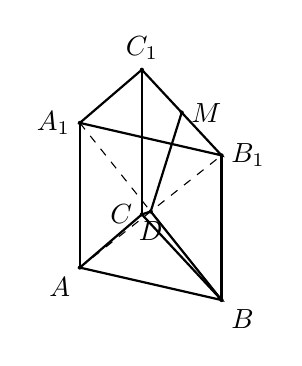
\begin{tikzpicture}[>=stealth,scale=0.75]
  \coordinate (A) at (0,0); \coordinate (B) at (2.4,-0.55);
  \coordinate (C) at (1.05,0.9); \coordinate (A1) at (0,2.45);
  \coordinate (B1) at (2.4,1.9); \coordinate (C1) at (1.05,3.35);
  \coordinate (D) at (1.2,0.95); \coordinate (M) at (1.725,2.625);
  \draw[thick] (A)--(B)--(C)--cycle;
  \draw[thick] (A1)--(B1)--(C1)--cycle;
  \draw[thick] (A)--(A1) (B)--(B1) (C)--(C1);
  \draw[dashed] (A)--(B1) (A1)--(B) (C)--(D);
  \draw[thick] (D)--(C) (D)--(B) (D)--(M);
  \fill (A) circle (1pt) node[below left] {$A$};
  \fill (B) circle (1pt) node[below right] {$B$};
  \fill (C) circle (1pt) node[left] {$C$};
  \fill (A1) circle (1pt) node[left] {$A_1$};
  \fill (B1) circle (1pt) node[right] {$B_1$};
  \fill (C1) circle (1pt) node[above] {$C_1$};
  \fill (D) circle (1pt) node[below] {$D$};
  \fill (M) circle (1pt) node[right] {$M$};
\end{tikzpicture}
\end{center}
\nopagebreak[4]
（1） 求证：$CD\perp$ 平面 $BDM$；

（2） 求面 $B_1BD$ 与面 $CBD$ 所成二面角的大小。

\end{question}
\begin{question}
\gkti{21}给定抛物线 $C:y^2=4x$，$F$ 是 $C$ 的焦点，过点 $F$ 的直线 $l$ 与 $C$ 相交于 $A\text{、}B$ 两点。

（1） 设 $l$ 的斜率为 $1$，求 $\overrightarrow{OA}$ 与 $\overrightarrow{OB}$ 夹角的大小；

（2） 设 $\overrightarrow{FB}=\lambda\overrightarrow{AF}$，若 $\lambda\in[4,9]$，求 $l$ 在 $y$ 轴上截距的变化范围。

\end{question}
\begin{question}
\gkti{22}已知函数 $f(x)=\ln(1+x)-x$，$g(x)=x\ln x$。

（1） 求函数 $f(x)$ 的最大值；

\Needspace{5\baselineskip}
（2） 设 $0<a<b$，证明：

\nopagebreak[4]
\[
0<g(a)+g(b)-2g\left(\frac{a+b}{2}\right)<(b-a)\ln2\text{。}
\]

\end{question}